\documentclass[10.5pt]{article}

\usepackage[margin=0.72in]{geometry}
\usepackage{amsmath,amssymb,booktabs,graphicx,microtype,xcolor,float}
\usepackage[hidelinks]{hyperref}
\usepackage[font=small,labelfont=bf]{caption}
\usepackage{enumitem}

\definecolor{atlasblue}{HTML}{176B87}
\definecolor{atlasorange}{HTML}{B66A1E}
\definecolor{atlasgray}{HTML}{4B5563}
\hypersetup{colorlinks=true,linkcolor=atlasblue,urlcolor=atlasblue}
\setlength{\parindent}{0pt}
\setlength{\parskip}{4.5pt}
\setlength{\emergencystretch}{3em}
\setlist[itemize]{leftmargin=1.25em,itemsep=1.5pt,topsep=2pt}
\newcommand{\fedd}{f_{\mathrm{Edd}}}
\newcommand{\mbh}{M_{\mathrm{BH}}}
\newcommand{\mseed}{M_{\mathrm{seed}}}
\newcommand{\repo}[1]{{\footnotesize\texttt{#1}}}

\title{\textbf{The High-Redshift Accretion Atlas}\\
\large A Tour of the Final Catalogue and Paper-Ready Results}
\author{Repository status document}
\date{2 September 2026}

\begin{document}
\maketitle

\begin{abstract}
This document is a guided tour of the repository's most significant scientific
products and the pipeline that produces them. Versions now identify nested
datasets rather than software releases. v1 is the complete analysis of the
original 23-object JADES broad-line AGN catalogue; v2 applies the same analysis
to 112 comparable broad-line AGN; and v3 is the final heterogeneous atlas of
234 measurements, 219 physical objects, and 218 host systems. Every version has
the same baseline evaluation, ranking, 10,000-sample Monte Carlo uncertainty,
duty-cycle, compatibility, and visual products. In v3, 196 objects support
numerical growth inference and 23 remain visible as explicit no-inference
cases. The figures are diagnostic comparisons under stated assumptions, not
evidence for a unique seed or accretion history.
\end{abstract}

\section{Start here: the three dataset views}

The central design rule is simple: changing version changes catalogue
membership, not the scientific question or the visual language.

\begin{table}[h]
\centering
\caption{Canonical dataset scopes and analysis coverage.}
\begin{tabular}{@{}llrrrr@{}}
\toprule
Version & Scope & Measurements & Objects & Hosts & Numeric objects \\
\midrule
v1 & Original JADES BLAGN & 23 & 23 & 23 & 23 \\
v2 & Expanded comparable BLAGN & 119 & 112 & 111 & 112 \\
v3 & Final heterogeneous atlas & 234 & 219 & 218 & 196 \\
\bottomrule
\end{tabular}
\end{table}

The canonical one-row-per-object tables live in
\repo{data/processed/v1/}, \repo{data/processed/v2/}, and
\repo{data/processed/v3/}; each is named
\repo{<version>\_accreting\_objects.csv}. The corresponding measurement tables
retain every literature measurement, including alternates of the same physical
object. Identity products in \repo{data/crossmatch/<version>/} record aliases,
preferred measurements, object-host links, and reviewed match decisions.

v2 groups the sources that use a comparable broad-line workflow: JADES,
Taylor CEERS/RUBIES, Matthee EIGER/FRESCO, Lin ASPIRE, Harikane NIRSpec,
Davis/THRILS, and Ren ALPINE/CRISTAL. v3 adds the object types that require
materially different handling: XQR-30 and GNIRS-50 luminous quasars, the UHZ1
X-ray evidence history, and the audited Scholtz narrow-line candidates.

\section{What is in the final catalogue?}

Figure~\ref{fig:landscape} is the quickest scientific overview. The left panel
shows every growth-eligible preferred object in redshift-mass space. The right
panel makes the analysis boundary explicit: objects without a supported
canonical mass stay in the catalogue instead of disappearing from the figure.

\begin{figure}[H]
\centering
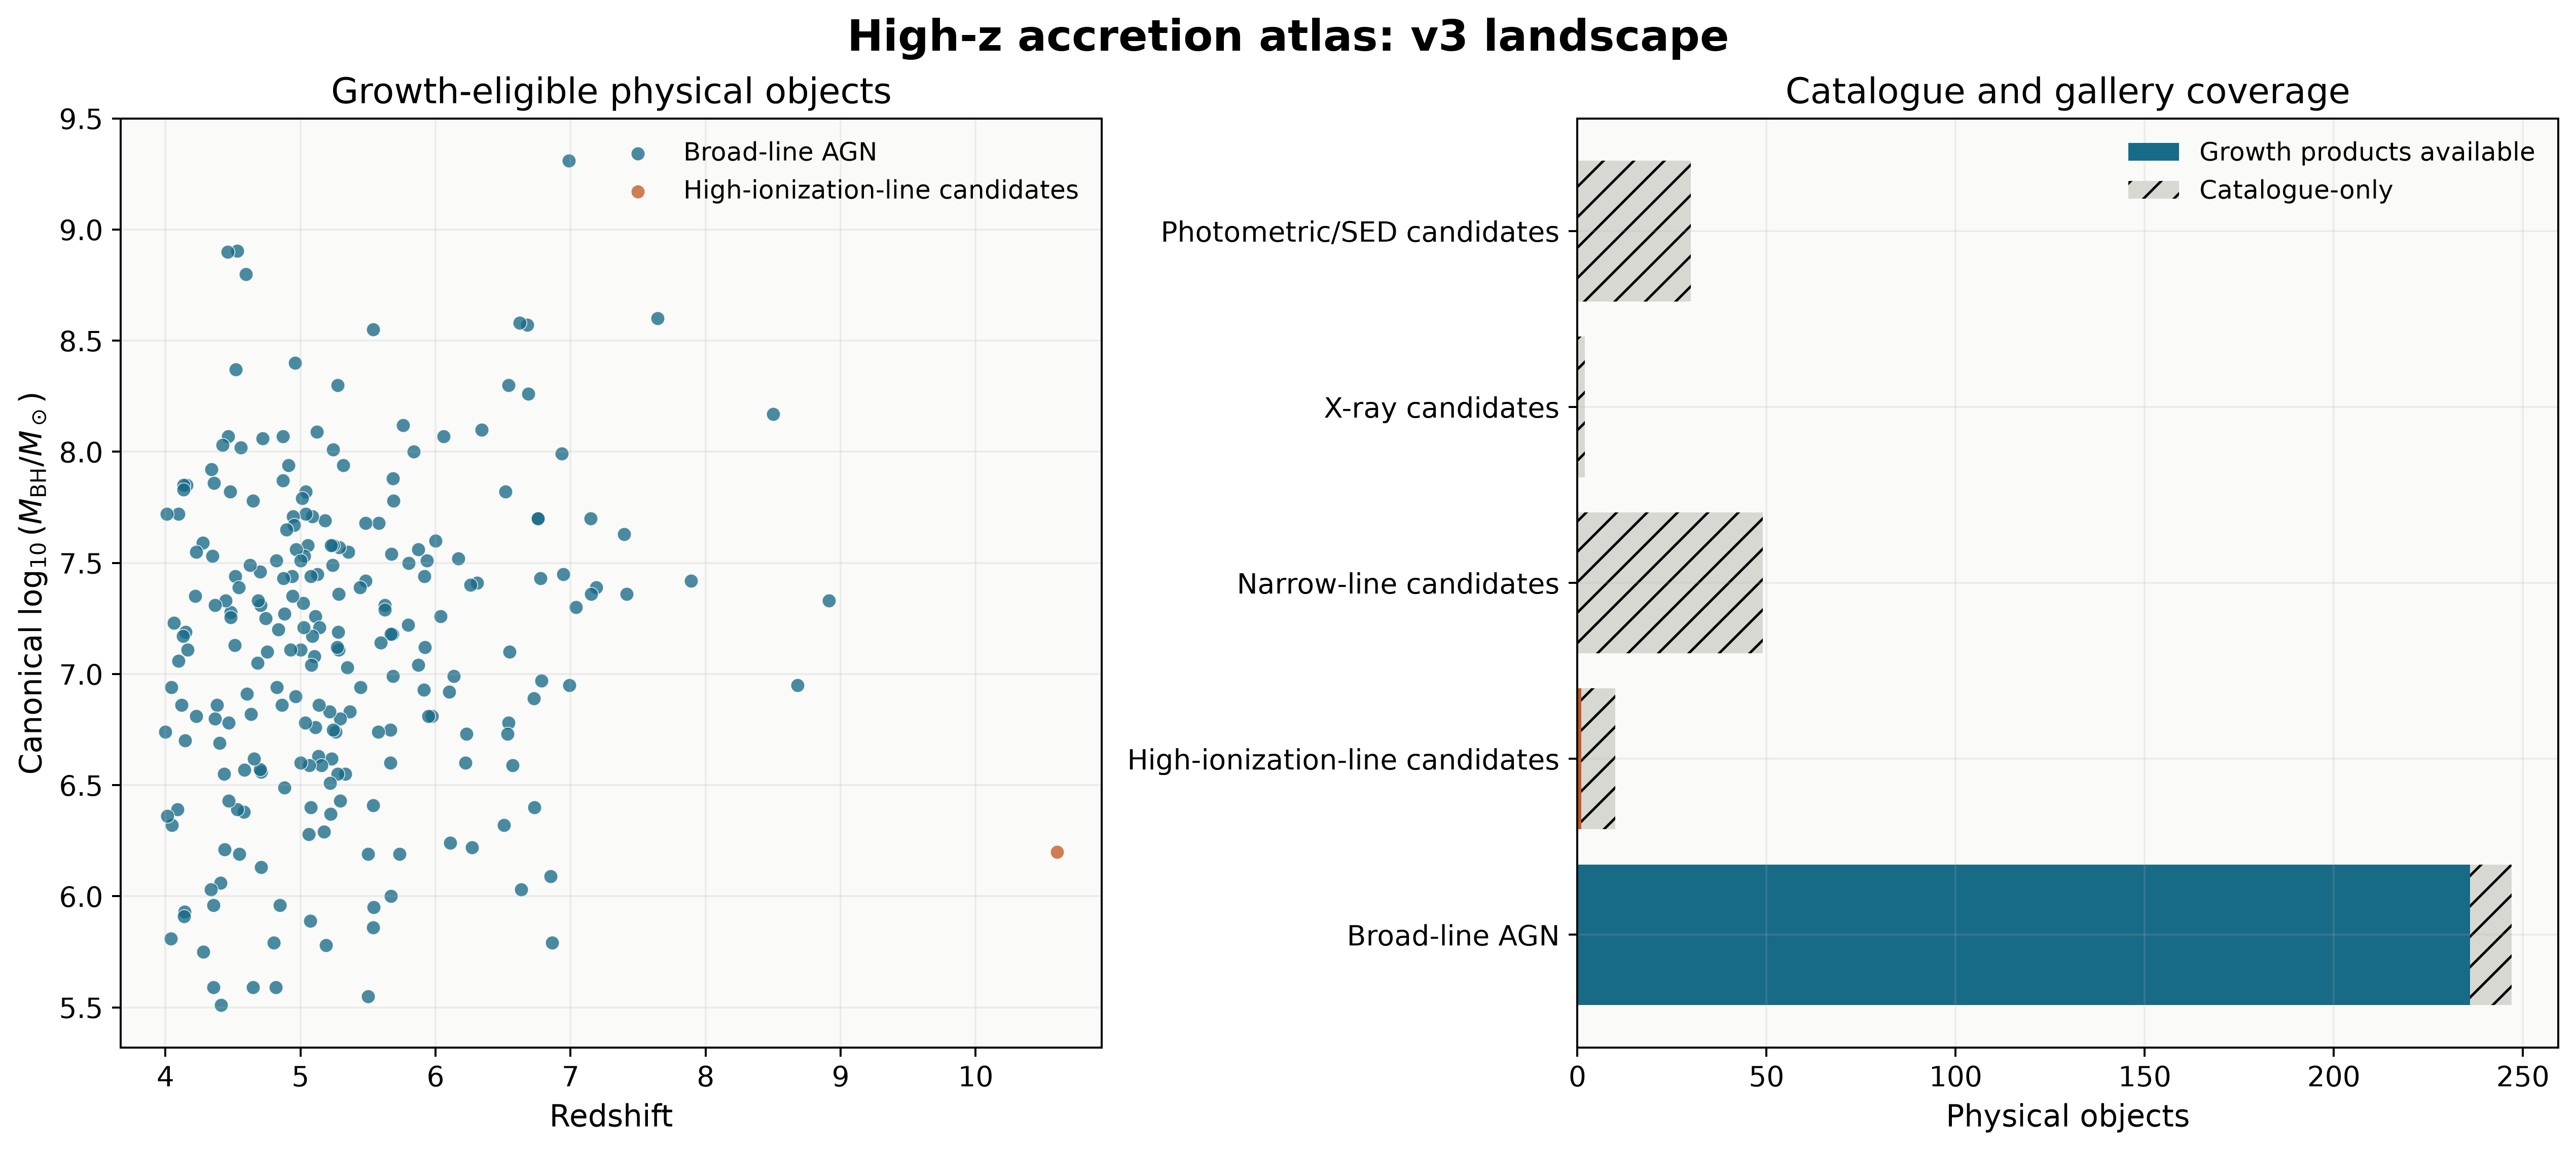
\includegraphics[width=0.98\textwidth]{../../../results/v3/figures/v3_catalogue_growth_landscape.png}
\caption{Final v3 catalogue landscape. The heterogeneous classes are kept
visually distinct, and catalogue-only objects are counted rather than assigned
an inferred mass.}
\label{fig:landscape}
\end{figure}

The final object composition is 112 broad-line AGN, 86 luminous-quasar
comparison objects, 20 narrow-line candidates, and one X-ray candidate. The
catalogue contains 219 unique physical objects even though it retains 234
measurements. This difference is scientifically useful: alternate measurements
are preserved for sensitivity tests, while one documented preferred row drives
each object-level result.

\textbf{How it was obtained.} Source-specific ingestion code preserves native
measurements and provenance. The shared catalogue layer then normalizes
vocabulary, resolves physical identities and hosts, applies the preferred-row
policy, and computes evidence, mass-comparability, lensing, conditional-mass,
and growth-eligibility fields. The public
\repo{scripts/00\_process\_catalogues.ipynb} notebook calls the tested
\repo{src/internal/process\_catalogues.py} implementation to materialize v1,
v2, and v3 from this one corrected pipeline.

\section{The physical calculation behind every result}

The atlas uses the Dayal-style exponential growth relation
\begin{equation}
\mbh(t_{\rm obs})=\mseed
\exp\left[\fedd\left(\frac{1-\epsilon}{\epsilon}\right)
\frac{\Delta t}{t_{\rm Edd}}\right] B_{\rm merge},
\end{equation}
with cosmic time from a flat Planck-style cosmology. The model is evaluated in
three directions: predict the final mass, solve for the required lifetime-average
$\fedd$ at fixed seed mass, and solve for the required seed mass at fixed
accretion history. The baseline ranking uses $z_{\rm seed}=30$,
$\epsilon=0.1$, and $B_{\rm merge}=1$.

Figure~\ref{fig:tracks} places the final masses against representative reference
tracks. It is a timing and scale diagnostic, not a fit. The lower strip shows
all 23 objects for which a numerical growth track is deliberately unavailable.

\begin{figure}[H]
\centering
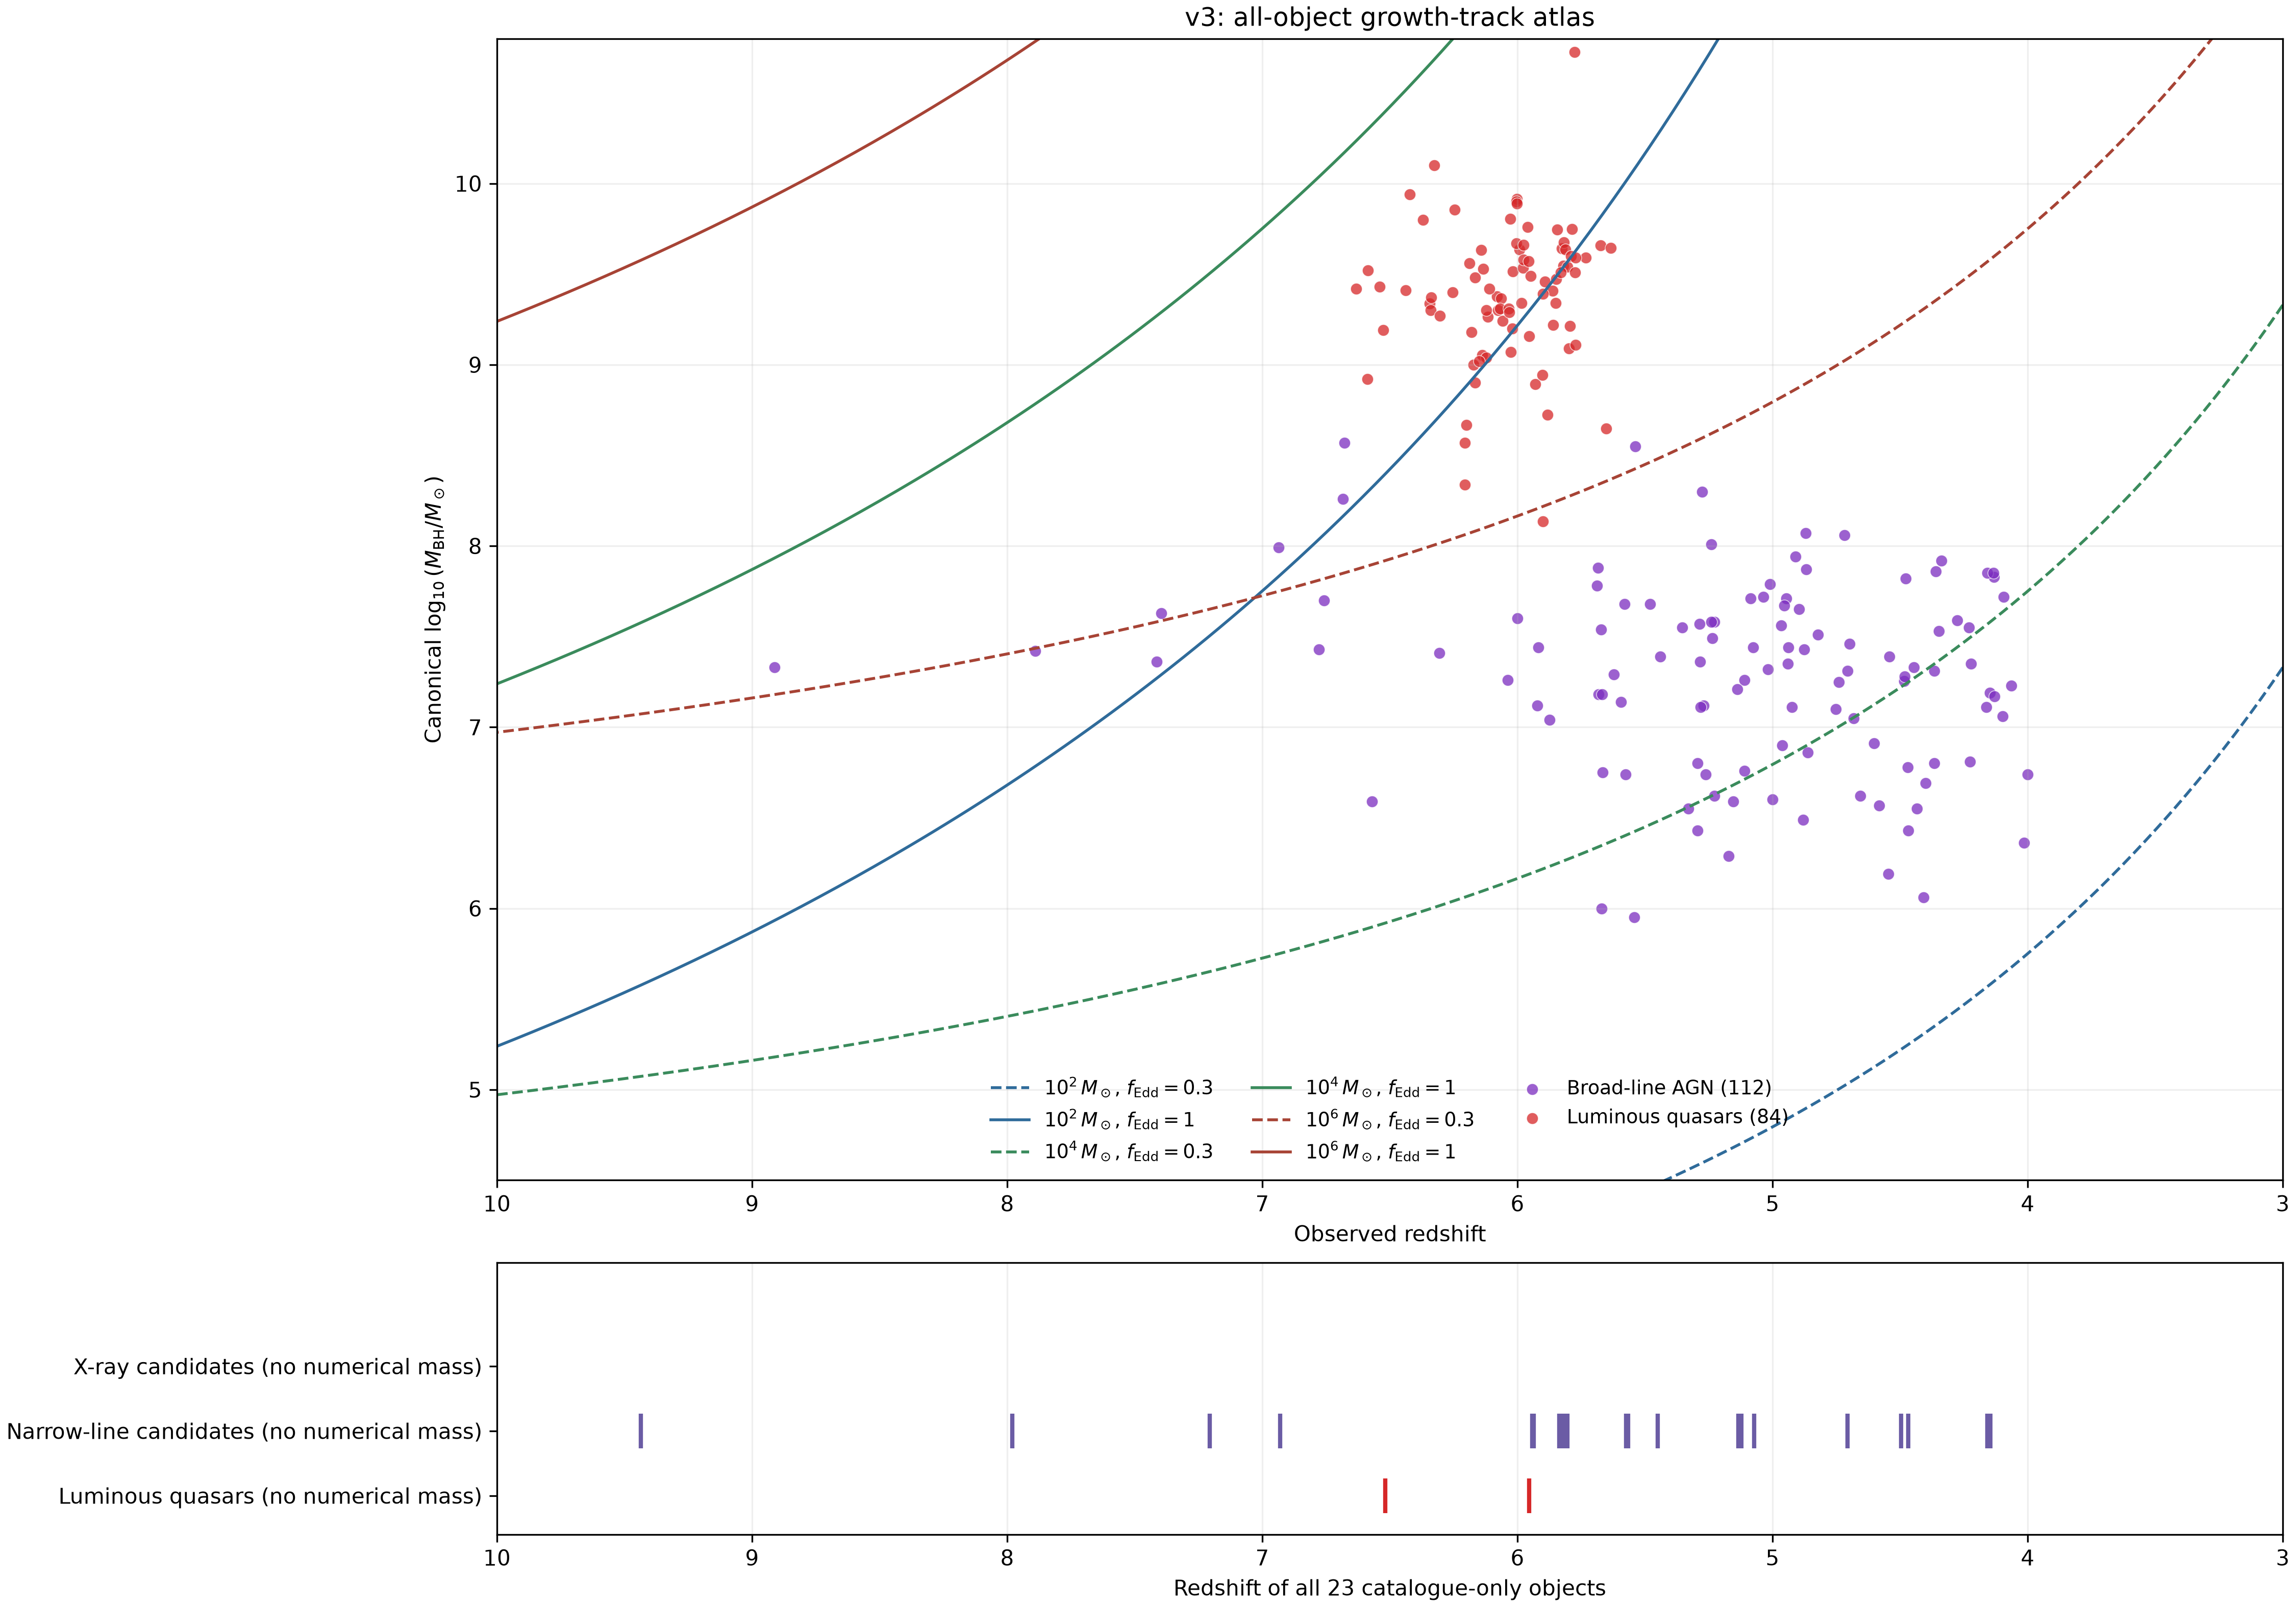
\includegraphics[width=0.98\textwidth]{../../../results/v3/figures/v3_all_object_growth_tracks.png}
\caption{All-object growth-track view. Supported masses appear above; every
unsupported object remains visible below with its class and redshift. The
common reversed redshift axis spans $z=10$ to $z=3$ with unchanged figure
dimensions and margins. Broad-line AGN are purple and luminous quasars are red.}
\label{fig:tracks}
\end{figure}

A separate
\href{../../../results/v3/figures/v3_all_object_growth_tracks_full_assumptions.png}
{comprehensive companion} preserves the historical v1 grid: three seed masses crossed with three
$f_{\rm Edd}$ values, four constant efficiencies, and two merger boosts, for
72 reference curves in total. It is an assumption comparison rather than a fit.
An
\href{../../../results/v3/figures/v3_all_object_growth_tracks_full_assumptions_uncertainty_filtered.png}
{uncertainty-filtered counterpart} keeps those curves but excludes the four luminous quasars with a maximum
reported black-hole-mass uncertainty above 0.7 dex. The reproducible selection
is stored in the
\href{../../../results/v3/tables/v3_growth_track_uncertainty_filter.csv}
{filter audit table}; the
canonical catalogue and rankings are unchanged.

The shared model also includes three Kerr spin cases, an illustrative
photon-trapping/slim-disk efficiency above Eddington, four seed families, and
a multiplicative merger boost. $B_{\rm merge}=2$ adds $\log_{10}2=0.301$ dex
to the final mass; it does not double the exponential accretion rate.

\section{Growth pressure: what is difficult under the baseline?}

The object ranking reports required parameters instead of a single opaque
compatibility score. Two central diagnostics are the required $\fedd$ for a
$10^2\,M_\odot$ seed and the required seed mass for lifetime-average
$\fedd=0.3$. The global ordering is a navigation aid only. Comparisons are
reported within object class and mass-comparability group, and pooled
demographic inference is explicitly disallowed.

\begin{figure}[H]
\centering
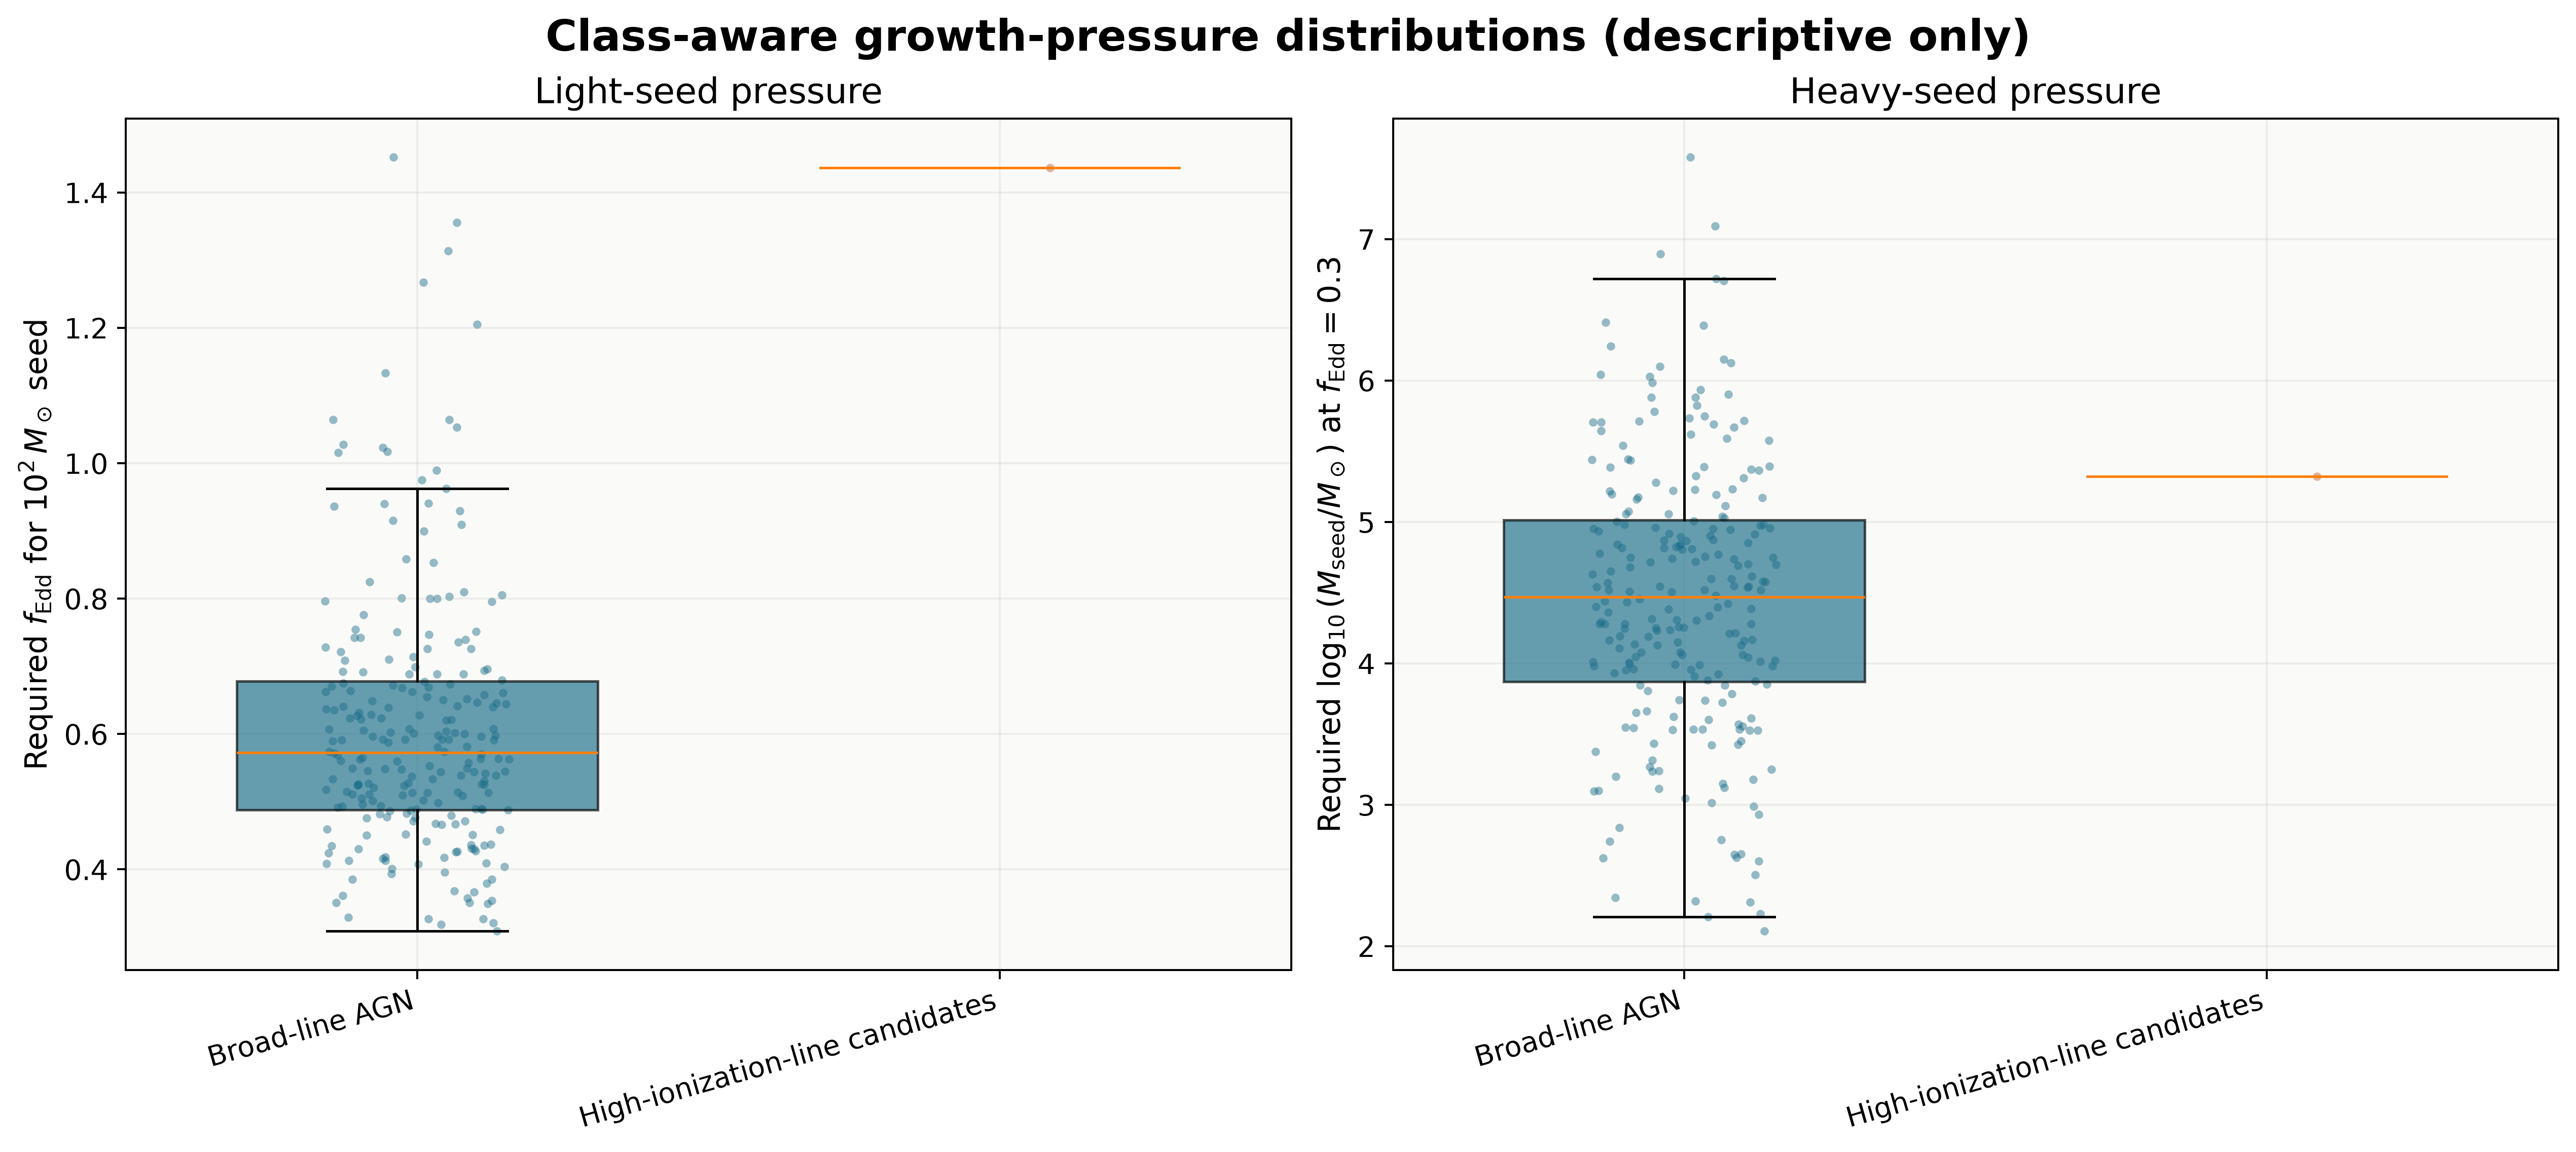
\includegraphics[width=0.98\textwidth]{../../../results/v3/figures/v3_class_aware_growth_pressure.png}
\caption{Class-aware distributions of the two baseline growth-pressure
diagnostics. The figure is descriptive because the source selections are not a
single complete population sample.}
\label{fig:pressure}
\end{figure}

In the original v1 sample, GN-38509 requires $\fedd=1.065$ for a
$10^2\,M_\odot$ seed and $\log_{10}(\mseed/M_\odot)=6.719$ for
$\fedd=0.3$. In the final v3 navigation view, the luminous quasar J1148+5251
is the highest point-pressure object, with required $\fedd=1.215$ and
$\log_{10}(\mseed/M_\odot)=7.980$ under the same baseline assumptions.
These values identify leverage under a coordinate system of assumptions; they
do not select one formation channel.

\textbf{Where to inspect it.} The complete baseline tables are
\repo{results/<version>/tables/<version>\_evaluation\_table.csv},
\repo{...\_required\_fedd\_by\_seed\_mass.csv}, and
\repo{...\_required\_mseed\_by\_growth\_assumption.csv}. Point rankings retain
the source, method, evidence, eligibility, and systematic-envelope metadata
beside every derived value.

\section{Uncertainty: which conclusions survive reported errors?}

For every eligible measurement and preferred object, the pipeline draws
10,000 deterministic samples from the reported asymmetric uncertainty in
$\log_{10}\mbh$. It recomputes the required $\fedd$ and seed mass for each
draw, storing percentile intervals and physically meaningful threshold
probabilities. Reported statistical errors are never blended with source-specific
virial systematics; systematic shifts remain separately labelled envelopes.

\begin{figure}[H]
\centering
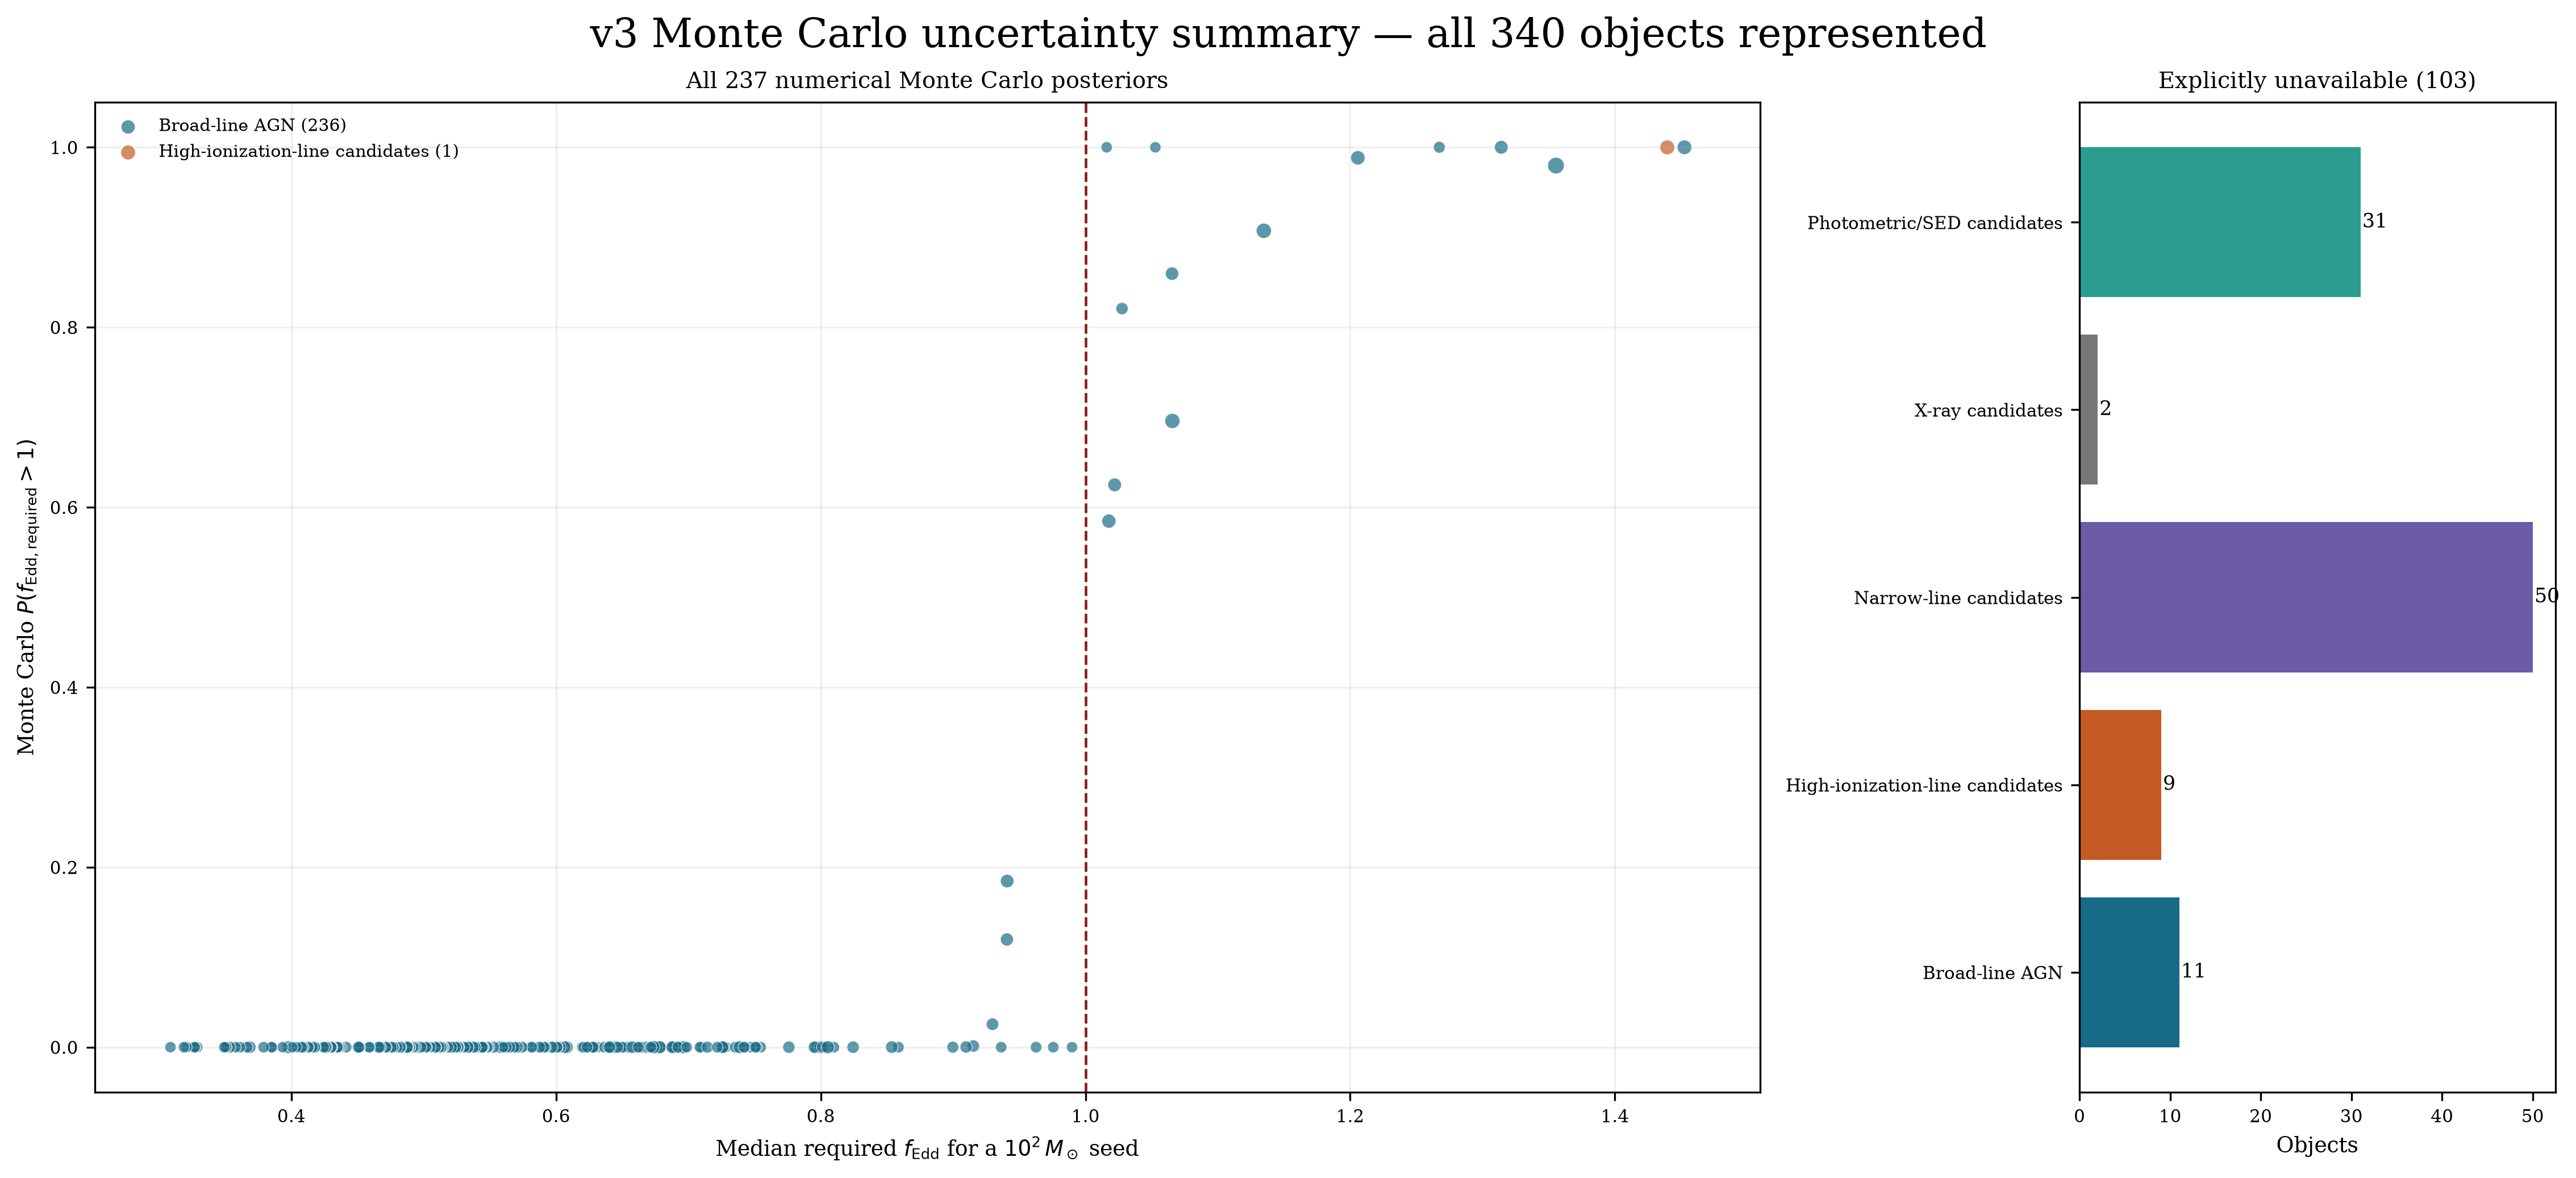
\includegraphics[width=0.98\textwidth]{../../../results/v3/figures/v3_monte_carlo_summary.png}
\caption{Monte Carlo summary for all 196 numerical v3 objects. Marker size
encodes interval width; the side panel accounts for the 23 objects that do not
support a numerical posterior.}
\label{fig:mc}
\end{figure}

The corresponding complete object atlas is
\repo{results/v3/figures/v3\_all\_object\_monte\_carlo\_uncertainty.png}.
In v1, GS-20057765 has a 0.980 posterior probability of requiring
$\fedd>1$ from a $10^2\,M_\odot$ seed under the baseline. Its tentative
detection status is retained next to that numerical pressure, preventing an
extreme value from being mistaken for an equally secure constraint.

The later science work also remains in every dataset version: effective
two-state histories with quiescent $\fedd=0$ and burst $\fedd=1,2,3$. The
stored duty cycle can exceed one, explicitly indicating that a fixed burst
scenario is insufficient. Published current Eddington ratios are treated as
instantaneous measurements and are not substituted for lifetime averages.

\textbf{How it was obtained.} \repo{scripts/01\_generate\_science.ipynb} calls
the shared class-aware Python engine for all three datasets. Object-stable random seeds
make the Monte Carlo tables reproducible when the catalogue is expanded.

\section{Compatibility: which assumption families can reach each object?}

Compatibility is evaluated object by object across four seed families, three
spin cases, two merger cases, and three lifetime-average Eddington ratios.
Figure~\ref{fig:compat} summarizes compatible fractions within each class;
the complete object-labelled matrix is stored beside it.

\begin{figure}[H]
\centering
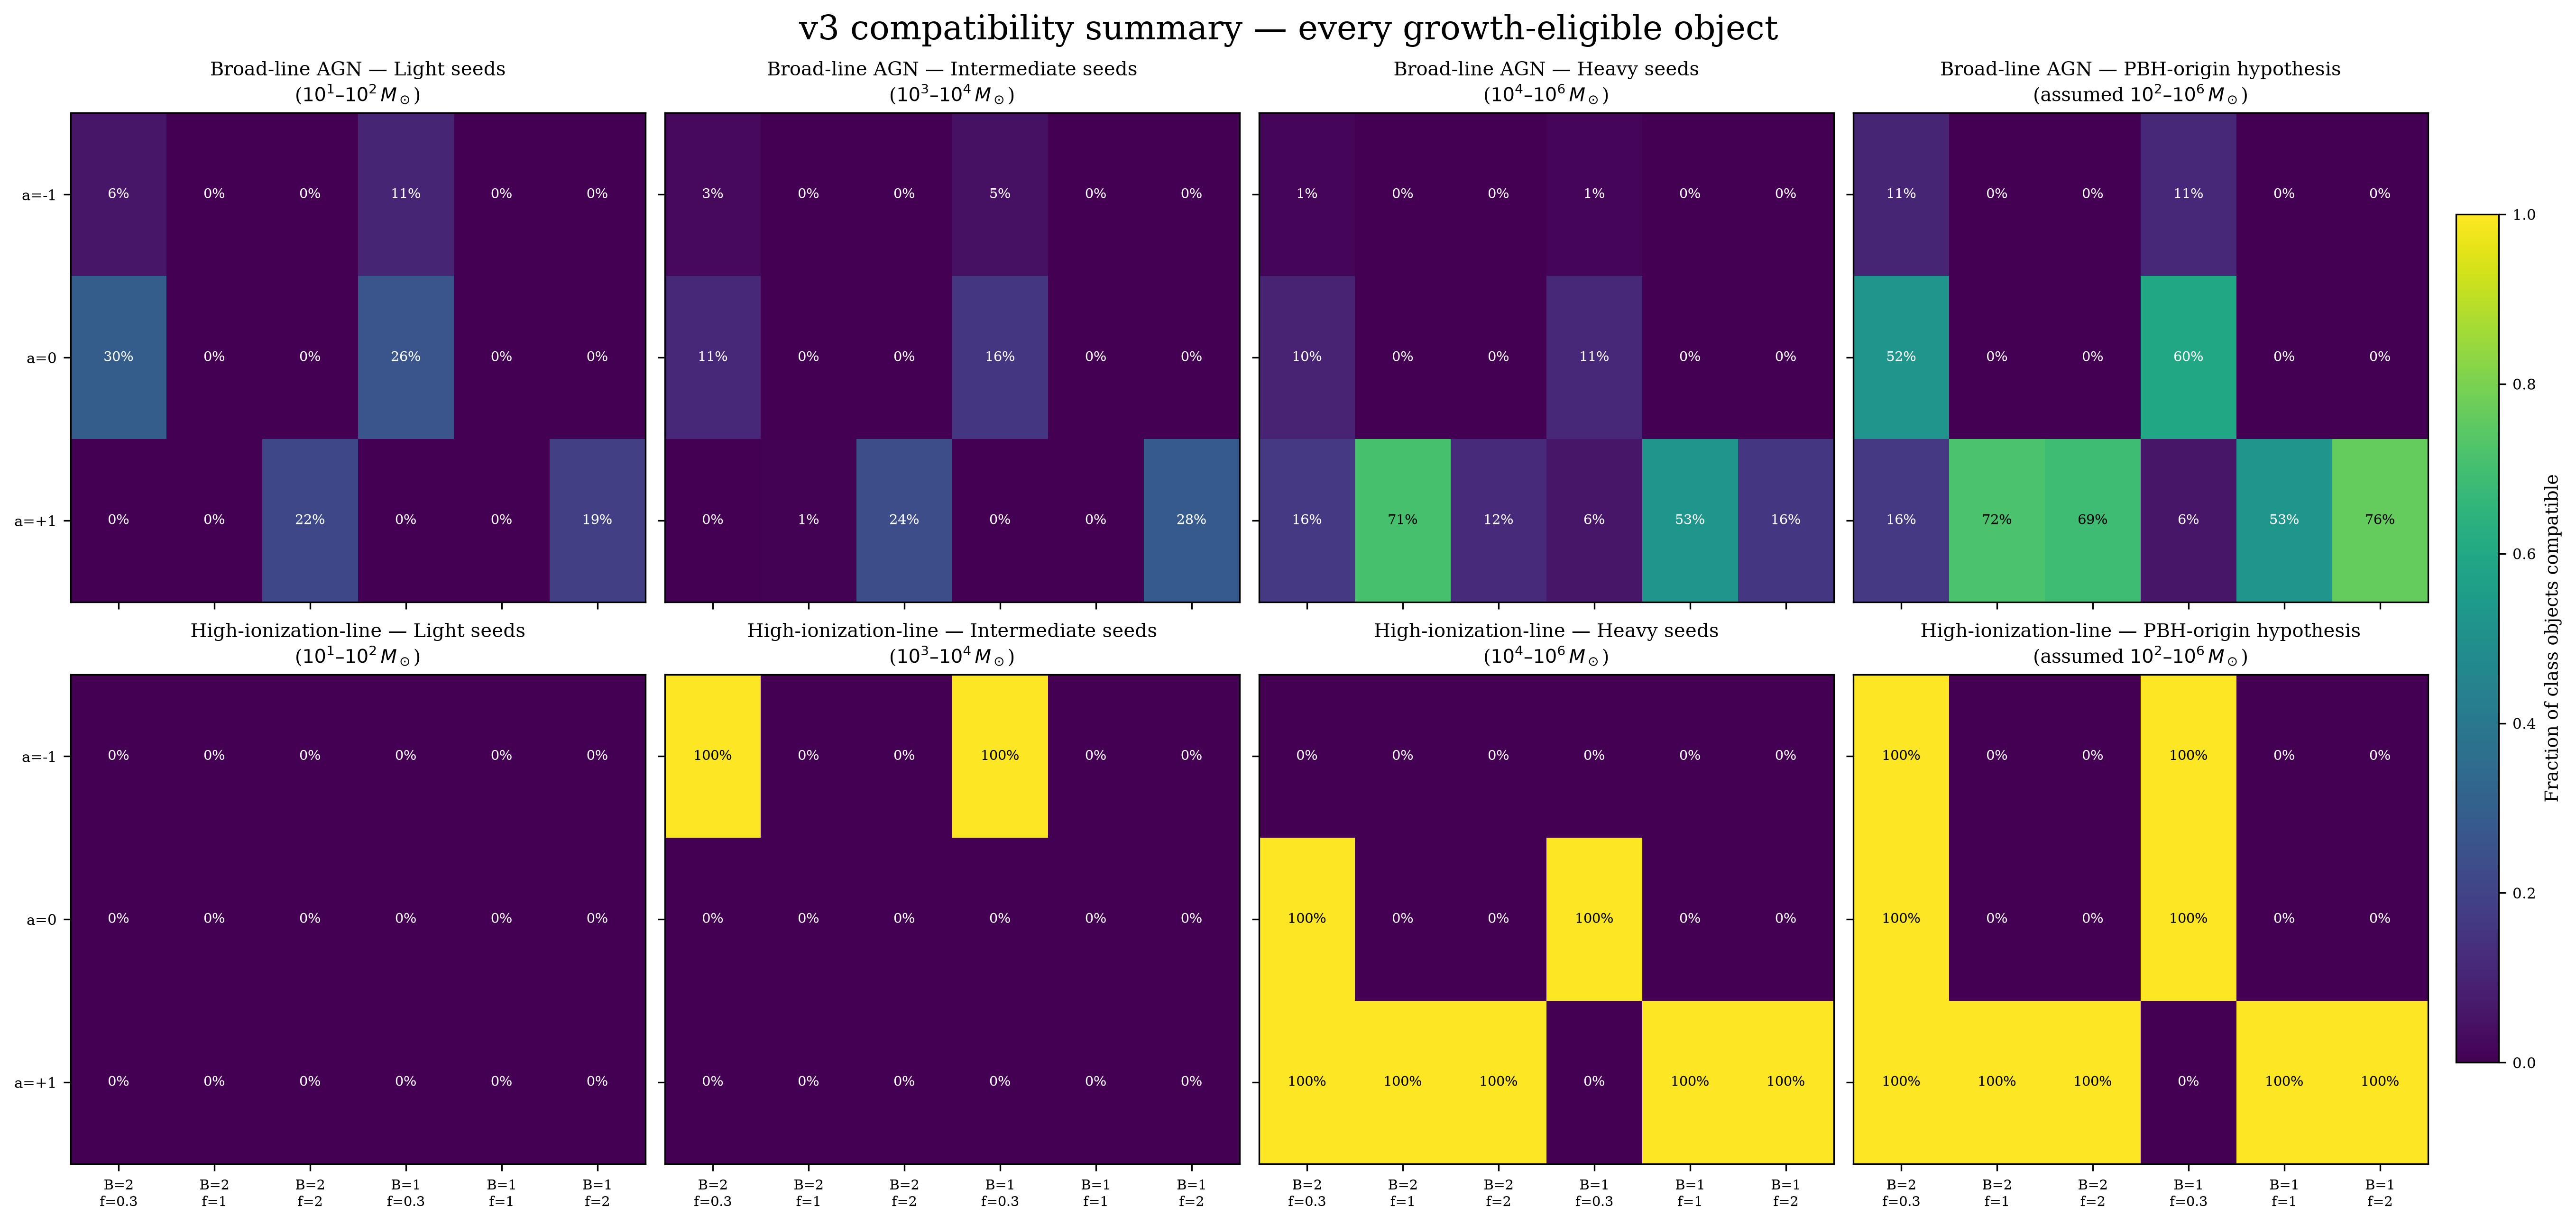
\includegraphics[width=0.98\textwidth]{../../../results/v3/figures/v3_compatibility_summary.png}
\caption{Class-specific compatibility fractions across seed, spin, merger,
and accretion assumptions. Fractions are descriptive within the observed
catalogue and are not occurrence rates.}
\label{fig:compat}
\end{figure}

The complete numerical table is
\repo{results/v3/tables/v3\_all\_object\_compatibility.csv}; it contains every
object-scenario combination. Unsupported objects have explicit unavailable
values rather than false incompatibilities. The full visual matrix is
\repo{results/v3/figures/v3\_all\_object\_compatibility\_atlas.png}.

\section{From catalogue scale to individual objects}

Each catalogue object receives two canonical gallery products: a parameter-map
sheet and a seed-redshift panel. The parameter sheet compares six spin/merger
combinations and uses the photon-trapping efficiency prescription where
appropriate. Figure~\ref{fig:object} shows the GN-38509 example. Equivalent
panels exist for every v1, v2, and v3 object.

\begin{figure}[H]
\centering
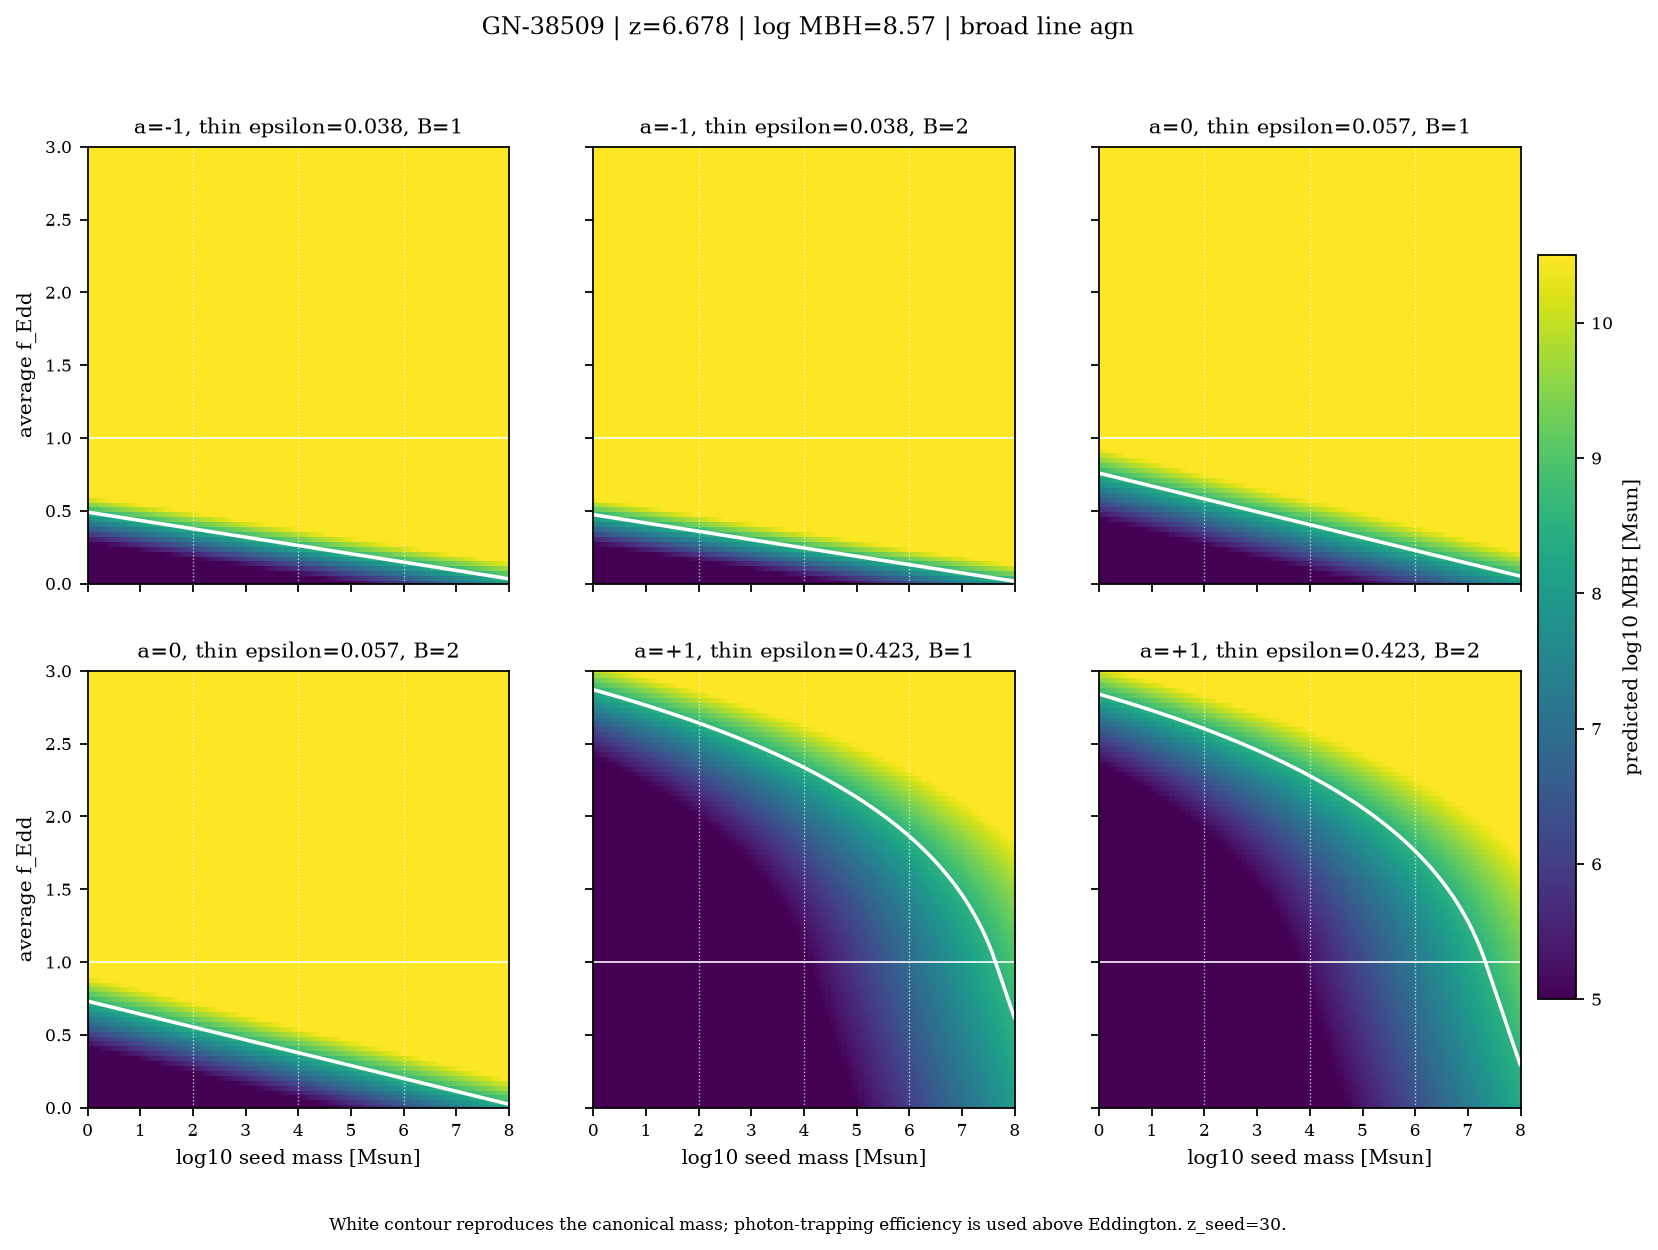
\includegraphics[width=0.98\textwidth]{../../../results/v3/gallery/fedd_mass_maps/v3_fedd_mass_map_hza-gn-38509.png}
\caption{GN-38509 parameter-map sheet. Color gives the predicted final
black-hole mass across seed mass and lifetime-average accretion rate. The
observed mass contour shows which combinations reproduce the preferred
measurement under each spin and merger case.}
\label{fig:object}
\end{figure}

The compiled v1 map gallery demonstrates that the original 23-object dataset
is complete in results rather than serving as a partial prototype. v2 and v3
use the identical panel definition at larger scale. For the 23 v3 objects
without a supported mass, the same file locations contain carefully labelled
status panels explaining why no numerical inference was made.

\textbf{Where to browse.} The per-object products are in the
\repo{fedd\_mass\_maps/} and \repo{seedredshift\_mass\_maps/} subdirectories
under \repo{results/<version>/gallery/}.
Catalogue-wide galleries are in \repo{results/<version>/figures/}. The visual
coverage CSV in the version's table directory links every object to both files
and distinguishes numerical products from no-inference panels.

\section{Measurement choice and provenance remain visible}

Thirteen eligible alternate measurements in v3 are compared against their
preferred object rows. The sensitivity plot shows how a literature-measurement
choice changes both $\log\mbh$ and the derived required $\fedd$ without
silently replacing either published value.

\begin{figure}[H]
\centering
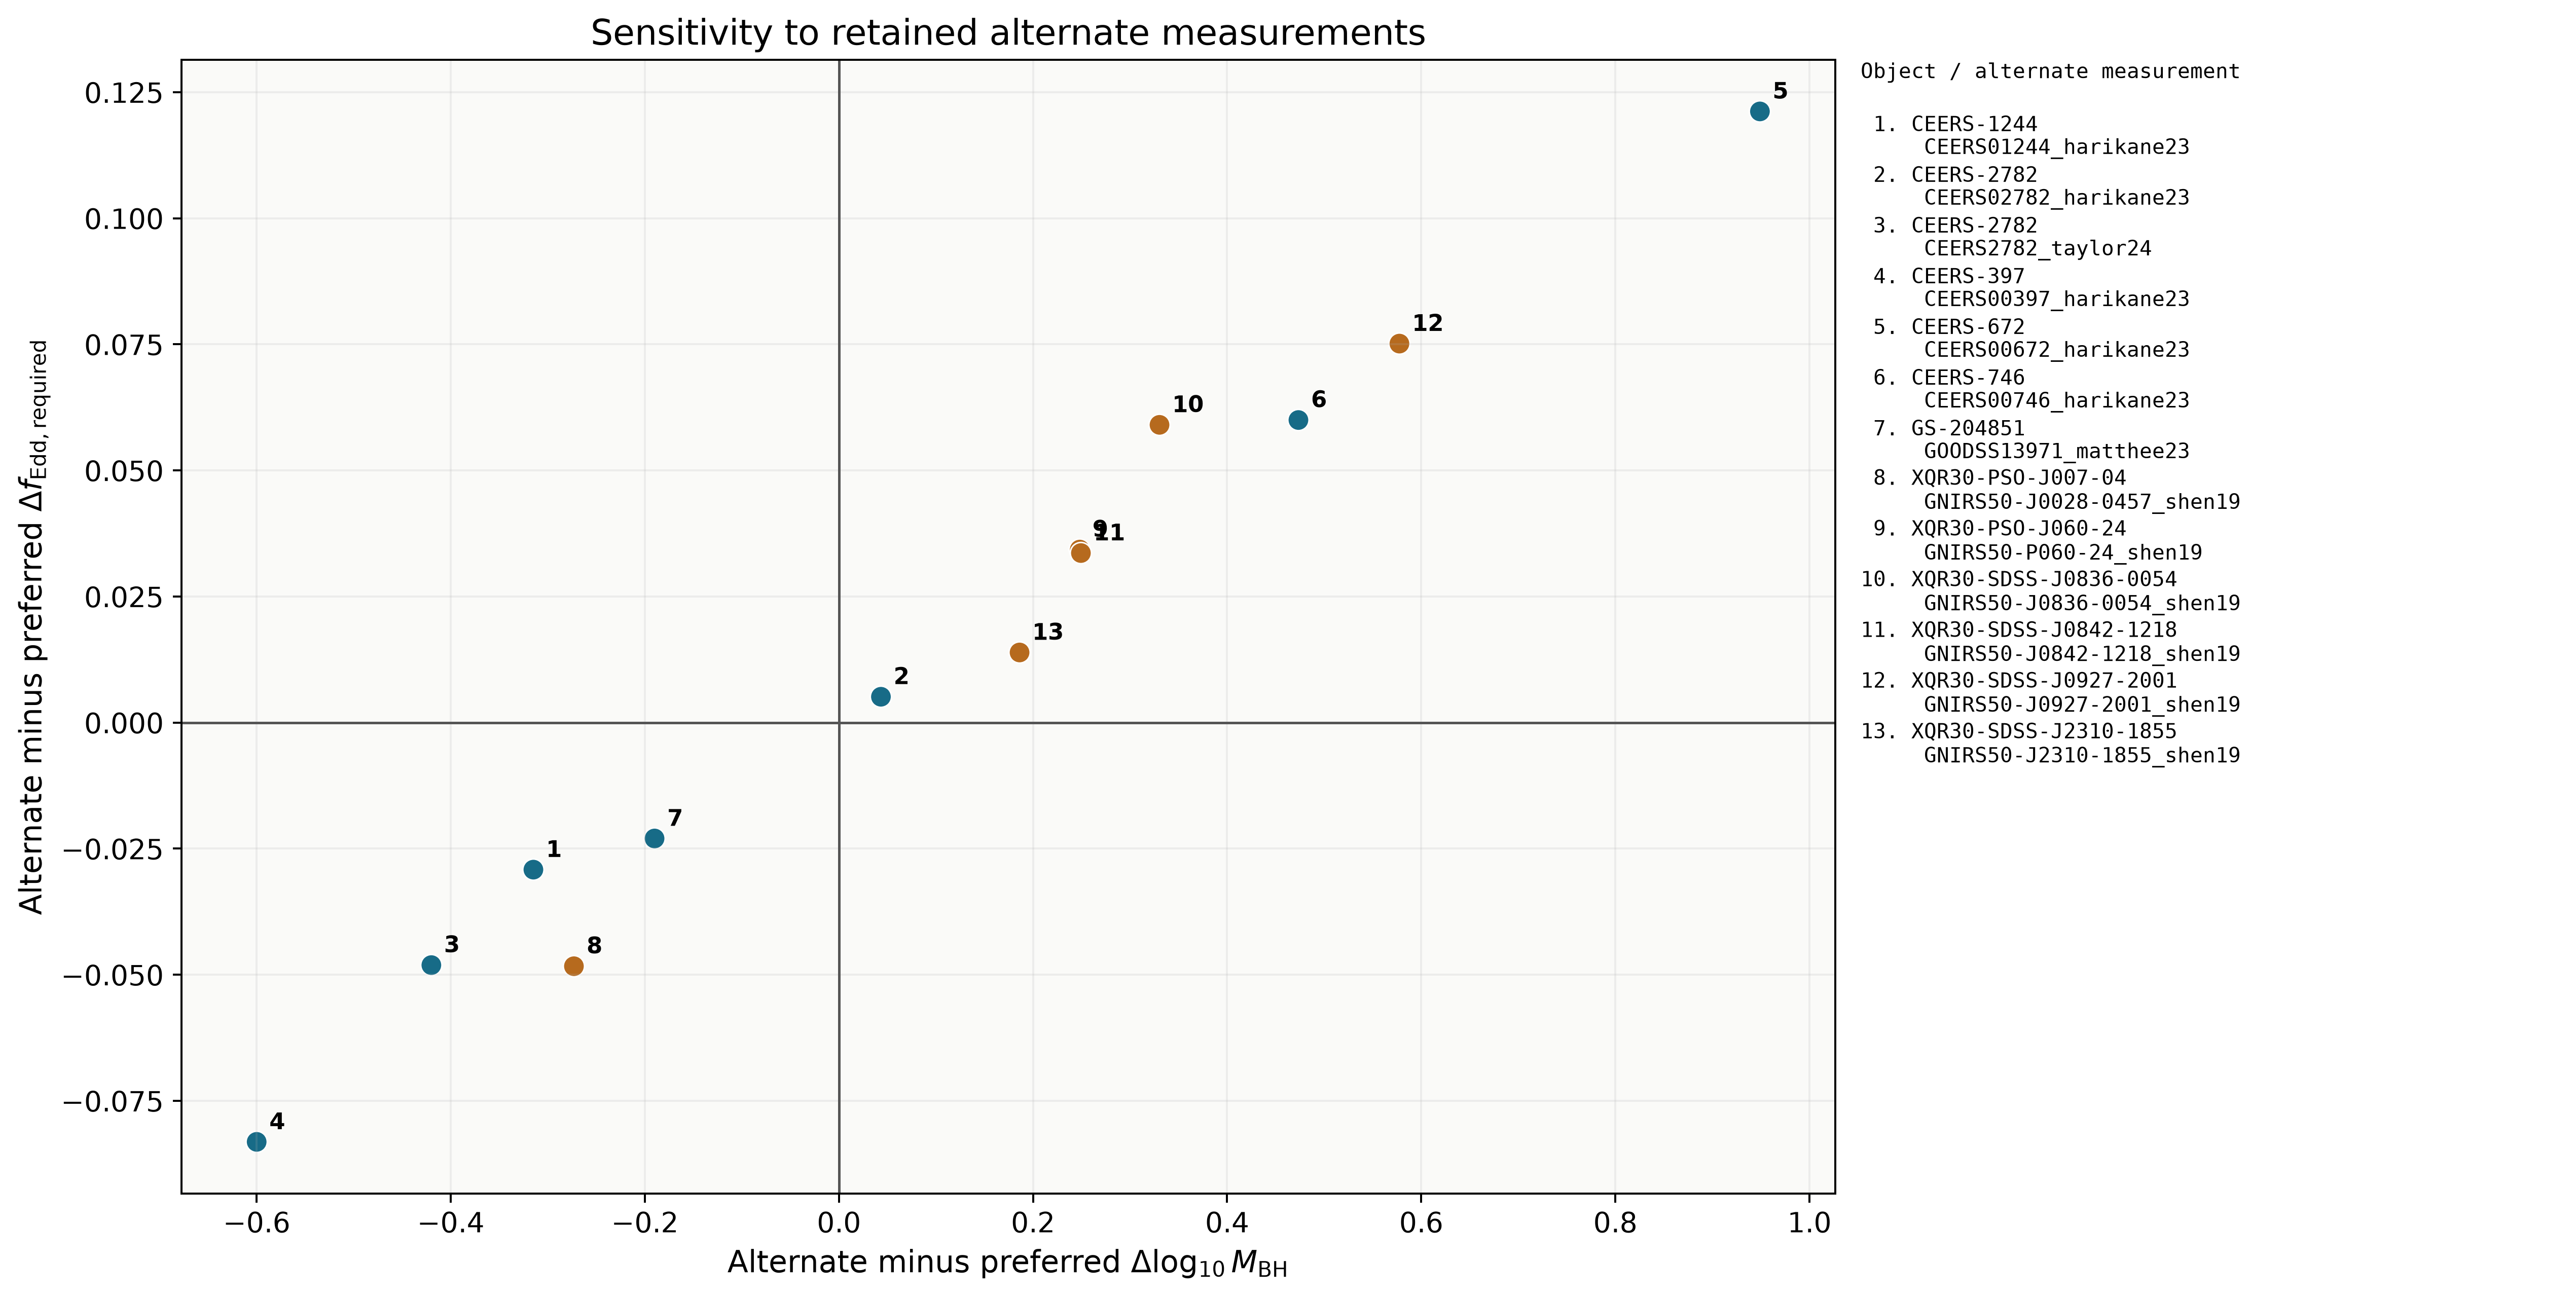
\includegraphics[width=0.96\textwidth]{../../../results/v3/figures/v3_measurement_sensitivity.png}
\caption{Sensitivity to retained alternate measurements. Numbered points map
to explicit object and measurement IDs in the side key and CSV table.}
\label{fig:sensitivity}
\end{figure}

Every scientific row can be traced to a source key, table, paper version, URL,
DOI/archive record, extraction status, method, and caveat. Identity decisions
are separate tables rather than hidden string matching. Preferred measurements
control object-level results, but all measurement-level evidence states and
values remain available for audit. The follow-up matrix retains all 219
objects, ranking 196 and leaving 23 explicitly unranked; the caveat summary
contains one row for each of the 11 admitted source families.

\section{Repository tour and exact reproduction}

The shortest path through the repository is:

\begin{enumerate}[leftmargin=1.5em,itemsep=3pt]
  \item \repo{docs/guides/versioning.md}: authoritative v1/v2/v3 membership.
  \item \repo{data/sources.md}: source-by-source extraction and caveats.
  \item \repo{data/processed/v3/v3\_accreting\_objects.csv}: final object view.
  \item \repo{src/datasets.py}: deterministic dataset materialization.
  \item \repo{src/models.py}: cosmology and black-hole growth equations.
  \item \repo{src/science.py}: shared rankings, uncertainty, and duty cycles.
  \item \repo{results/v3/tables/}: complete numerical paper and audit products.
  \item \repo{results/v3/figures/}: paper-ready summaries and complete atlases.
  \item \repo{results/v3/gallery/fedd\_mass\_maps/} and
  \repo{results/v3/gallery/seedredshift\_mass\_maps/}: the full visual supplement.
  \item \repo{scripts/04\_verify.ipynb}: public verification workflow.
  \item \repo{src/internal/verify\_versions.py}: manifests, result inventory,
  exact CSV reproduction, counts, nesting, samples, compatibility, image
  resolution, and per-object coverage checks.
\end{enumerate}

Reproduce the canonical products from the repository root:

\begin{verbatim}
mkdir -p /tmp/highz-atlas-notebooks
.venv/bin/jupyter nbconvert --to notebook --execute --output-dir=/tmp/highz-atlas-notebooks
  scripts/00_process_catalogues.ipynb
.venv/bin/jupyter nbconvert --to notebook --execute --output-dir=/tmp/highz-atlas-notebooks
  scripts/01_generate_science.ipynb
.venv/bin/jupyter nbconvert --to notebook --execute --output-dir=/tmp/highz-atlas-notebooks
  scripts/02_generate_figures.ipynb
.venv/bin/jupyter nbconvert --to notebook --execute --output-dir=/tmp/highz-atlas-notebooks
  scripts/03_generate_atlas.ipynb
.venv/bin/jupyter nbconvert --to notebook --execute --output-dir=/tmp/highz-atlas-notebooks
  scripts/04_verify.ipynb
\end{verbatim}

The verification contract requires strict nested membership
$\mathrm{v1}<\mathrm{v2}<\mathrm{v3}$, the expected 23/112/219 object counts,
10,000 samples in Monte Carlo and duty-cycle products, complete compatibility
tables, an exact result inventory, two visual panels per object, and
publication-resolution PNGs. The
broader regression suite and source-provenance and manuscript checks protect
the ingestion details and final claims.

\section{Interpretation boundary and status}

The project now has a coherent paper-ready endpoint. Its central deliverable is
not one favored black-hole seed model; it is a traceable map from reported
measurements and evidence states to the growth assumptions each object would
require. The strongest conclusions are therefore comparative:

\begin{itemize}
  \item which objects remain demanding after reported mass uncertainty;
  \item which conclusions depend on source method, alternate measurement, or
  conditional evidence;
  \item which seed/accretion families are compatible under explicit spin and
  merger assumptions; and
  \item which observations would most change the physical interpretation.
\end{itemize}

The important limitations remain explicit. The catalogue mixes selection
functions and cannot support pooled demographic rates. Virial systematics are
not complete posterior models. Duty-cycle scenarios are effective histories,
not reconstructed light curves. Candidate and disputed objects remain useful
for observational triage but are not promoted to secure constraints by a high
growth-pressure score.

Within those boundaries, v1 is complete in results, v2 demonstrates clean
scaling across comparable objects, and v3 is the final processed catalogue and
visual atlas for the source-family review cutoff of 27 August 2026. Relevant
but not-yet-admitted sources are recorded in
\repo{docs/current/literature-scope.md} and require a new dataset version.
Every significant paper-facing claim can be followed backward
from figure to table, preferred measurement, identity decision, and source.

\end{document}
